\documentclass{beamer}
% \usepackage{lmodern}
%=====================================================================
% Color definition
\definecolor{jvagreen}{RGB}{0,104,	139}
\definecolor{jvagold}{RGB}{255, 255, 255}
\setbeamercolor{section in head/foot}{fg = jvagold, bg = jvagreen}
\usepackage{graphicx}
\usepackage{mathtools}
\usepackage{picture}
\usepackage{amsmath}
\usepackage{multimedia}
\DeclareMathOperator{\Tr}{Tr}
%\graphicspath{{../}}
\setbeameroption{show notes}
\usepackage{multicol}
\usepackage{caption}
\usepackage{subcaption} % To use subfigures with subcaptions
\usepackage{textpos}

\captionsetup[subfigure]{labelformat=empty}
\renewcommand{\figurename}{}
\usepackage[labelsep=endash]{caption}

\usepackage{wrapfig}
\definecolor{light-gray}{gray}{0.95}
\usepackage{tcolorbox}

\newcommand{\phim}{\mathbf{\phi}}
\newcommand{\X}{\mathbf{X}}
\newcommand{\x}{\mathbf{x}}
\newcommand{\Y}{\mathbf{Y}}
\newcommand{\y}{\mathbf{y}}
\newcommand{\w}{\mathbf{w}}
\newcommand{\Z}{\mathbf{Z}}
\newcommand{\z}{\mathbf{z}}
\newcommand{\h}{\mathbf{h}}
\newcommand{\dd}{\: \mathrm{d}}
\newcommand{\B}{\mathbf{B}}
\newcommand{\F}{\mathbf{F}}
\newcommand{\bb}{\mathbf{b}}
\newcommand{\vect}[1]{\mathbf{#1}}

\usebackgroundtemplate
{
    
\includegraphics[width=\paperwidth,height=\paperheight]{img/blank.jpg}%
}
\beamertemplatenavigationsymbolsempty

%=====================================================================
% Templates - headline, frametitle

\makeatletter
% Komprimiert die miniframe Kreise auf eine Linie
\beamer@compresstrue
\makeatother

% Definiert die headline
\setbeamertemplate{headline}
{ 
%\includegraphics[width=\paperwidth]{pic} % test logo
\begin{beamercolorbox}[wd=\paperwidth,right]{section in head/foot}
    \rule{\paperwidth}{1pt}
    %Vertikaler Abstand
    \vskip20pt
    %Fügt die Standard-Navi ein (miniframes)
    %\insertnavigation{\paperwidth}
    \vskip8pt
    %\rule{\paperwidth}{0.5pt}
    %\vskip25.5pt % same height of the example provided, but IMHO is too much
    \rule{\paperwidth}{1pt}
\end{beamercolorbox} 
}
\setbeamertemplate{footline}
{ 
%\includegraphics[width=\paperwidth]{pic} % test logo
\begin{beamercolorbox}[wd=\paperwidth,right]{section in head/foot}
    \rule{\paperwidth}{1pt}
    %Vertikaler Abstand
    \vskip10pt
    %Fügt die Standard-Navi ein (miniframes)
    \insertnavigation{\paperwidth}
    \vskip8pt
    \rule{\paperwidth}{0.5pt}
    %\vskip25.5pt % same height of the example provided, but IMHO is too much
    %\rule{\paperwidth}{1pt}
\end{beamercolorbox} 
}

% definition of the frametitle
\setbeamertemplate{frametitle}
{
\vskip-24pt % to shift up the frametitle
\hbox{ 
 \begin{beamercolorbox}[wd=.0675\textwidth]{} % left shift
 \end{beamercolorbox} 
 \begin{beamercolorbox}[sep=4pt]{section in head/foot}
 \insertframetitle
 \end{beamercolorbox} 
 }
}

\mode<presentation>
{
    \setbeamertemplate{itemize item}[circle]
    \setbeamercolor{itemize item}{fg = jvagreen}
    \setbeamertemplate{itemize subitem}[circle]
    \setbeamercolor{itemize subitem}{fg = jvagreen}
}

\renewcommand\footnoterule{}

\AtBeginSection[]
{
  \begin{frame}<beamer>
    \frametitle{Outline}
    \tableofcontents[currentsection]
  \end{frame}
}

%\logo{\includegraphics[height=0.6cm]{img/cde_basic_green}}
%\let\oldequation=\equation
%\let\endoldequation=\endequation
%\renewenvironment{equation}{\vspace{1cm}\begin{oldequation}}{\end{oldequation}\vspace{15mm}}

\begin{document}

\addtobeamertemplate{frametitle}{}{%
\begin{textblock*}{100mm}(-0.9cm,-0.6cm)

\includegraphics[height=0.5cm,width=1.5cm]{img/uob-logo-white-transparent}
\end{textblock*}
\begin{textblock*}{100mm}(0.97\textwidth,-0.6cm)

\includegraphics[height=0.5cm,width=1cm]{img/cde_tag_white}
\end{textblock*}
}

\title[Performance-driven Facial Animation]{
  Performance-driven Facial Animation}

% Optional: a subtitle to be dispalyed on the title slide
% \subtitle{Show where you're from}
% \subtitle{Presented by: Ieva Kazlauskaite}
% The author(s) of the presentation:
%  - again first a short version to be displayed at the bottom;
%  - next the full list of authors, which may include contact information;
\author[Garoe Dorta Perez, Ieva Kazlauskaite, Richard Shaw]{
   Garoe Dorta Perez, Ieva Kazlauskaite, Richard Shaw } 


% The institute:
%  - to start the name of the university as displayed on the top of each slide
%    this can be adjusted such that you can also create a Dutch version
%  - next the institute information as displayed on the title slide
\institute[University of Bath]{
University of Bath \\
Centre For Digital Entertainment
}

% Add a date and possibly the name of the event to the slides
%  - again first a short version to be shown at the bottom of each slide
%  - second the full date and event name for the title slide

\date{27 May 2015}

% TITLE PAGE
\begin{frame}[plain]
  \titlepage
\end{frame}

%\section{Overview}
% CONTENT PAGE
%\begin{frame}
%  \frametitle{Overview}
%  \tableofcontents
%\end{frame}

%----------------------------------------------------------------------
\section{Richard's Part}
\begin{frame}{Frame name}

\end{frame}

\begin{frame}{Frame name}

\end{frame}

%----------------------------------------------------------------------
\section{Blendshape Model}
\begin{frame}{General idea}
Given a set of blendshapes $\mathbf{B} = [\bb_1, \ldots, \bb_n]$ and a neutral face $\bb_0$, a new facial expression $\mathbf{F(\w)}$ is a linear combination of the offsets of the basic shapes:
\begin{equation*}
	\underbrace{\F(\w)}_{\text{new expression}} = \underbrace{ \bb_0 }_{\text{neutral face}}+ \sum_{i=1}^N \: \underbrace{w_i}_{\text{weights}} \: \underbrace{|\bb_i - \bb_0|}_{\text{offsets from neutral}}.
\end{equation*}
The \textbf{weights} describe how much each of the basic shapes affect the new expression. 
\end{frame}


\begin{frame}{Designing blendshapes}
\begin{description}
	\item[Option 1] Create blendshapes \textbf{by hand} $\Rightarrow$ correspond to a basic facial expression, for example a raised eyebrow.\\
					$\times$  Hard to produce. \vspace{0.5 cm}
	\item[Option 2] Use \textbf{P}rincipal \textbf{C}omponent \textbf{A}nalysis $\Rightarrow$ automatic construction. \\
					$\times$  Hard to adjust manually.
\end{description}

\end{frame}


\begin{frame}{Estimating weights}
The weights $\w$ are estimating by solving the following:


\begin{minipage}[t]{0.95\linewidth} 
\begin{tcolorbox}[colback=gray!5,colframe=jvagreen, title=Minimisation problem]
\begin{equation*}
	\min_\w \| \underbrace{\hat{\mathbf{B}}}_{\text{matrix with offsets}} \: \: \: \underbrace{\w}_{\text{vector of weights}} - \underbrace{(\F(\w) - \bb_0)}_{\text{offsets of new expression}} \|,
\end{equation*}        
\end{tcolorbox} 
\end{minipage}  \vspace{0.5 cm}

where the weights add up to $1$.

\end{frame}

\begin{frame}{Improvements}
\begin{itemize}
	\item Reduced set of blendshapes.
	\item Corrective shapes.
\end{itemize}

\end{frame}

\begin{frame}{Different Approaches}
\visible<1->{\begin{figure}
        \centering
        \begin{subfigure}[b]{0.43\textwidth}
                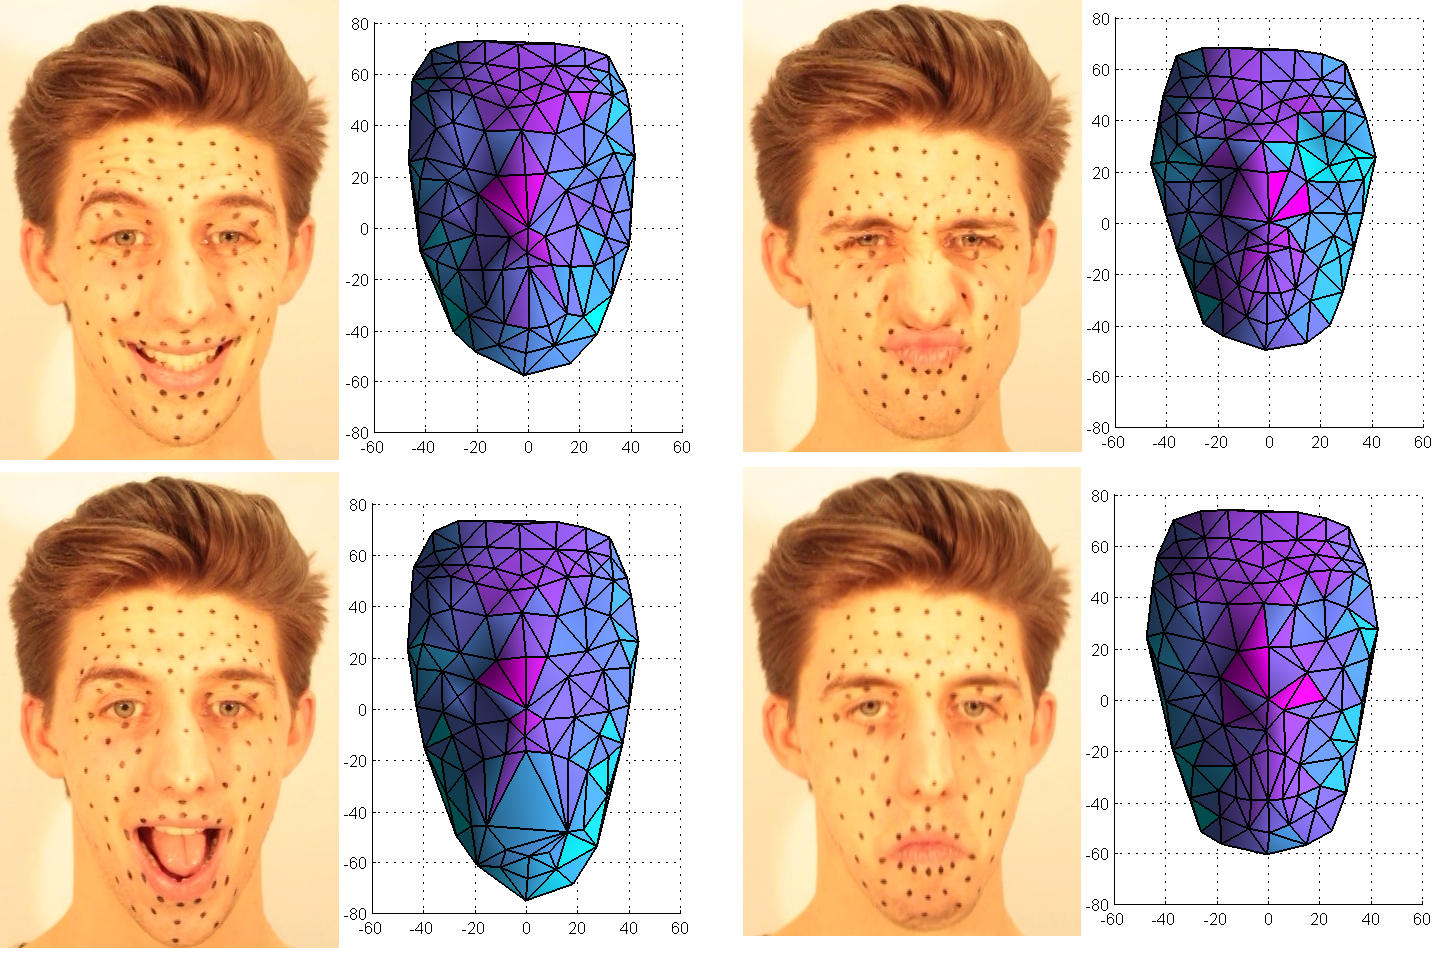
\includegraphics[width=\textwidth]{img/Richdomain}
                \caption{Recorded sequence}
        \end{subfigure}
        \begin{subfigure}[b]{0.2\textwidth}
                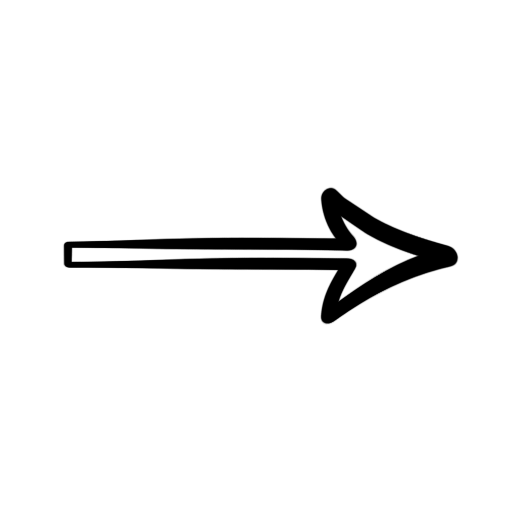
\includegraphics[width=\textwidth]{img/arrow}
                \caption{\hspace{0.2cm} Thin plate splines}
        \end{subfigure}
        \begin{subfigure}[b]{0.3\textwidth}
                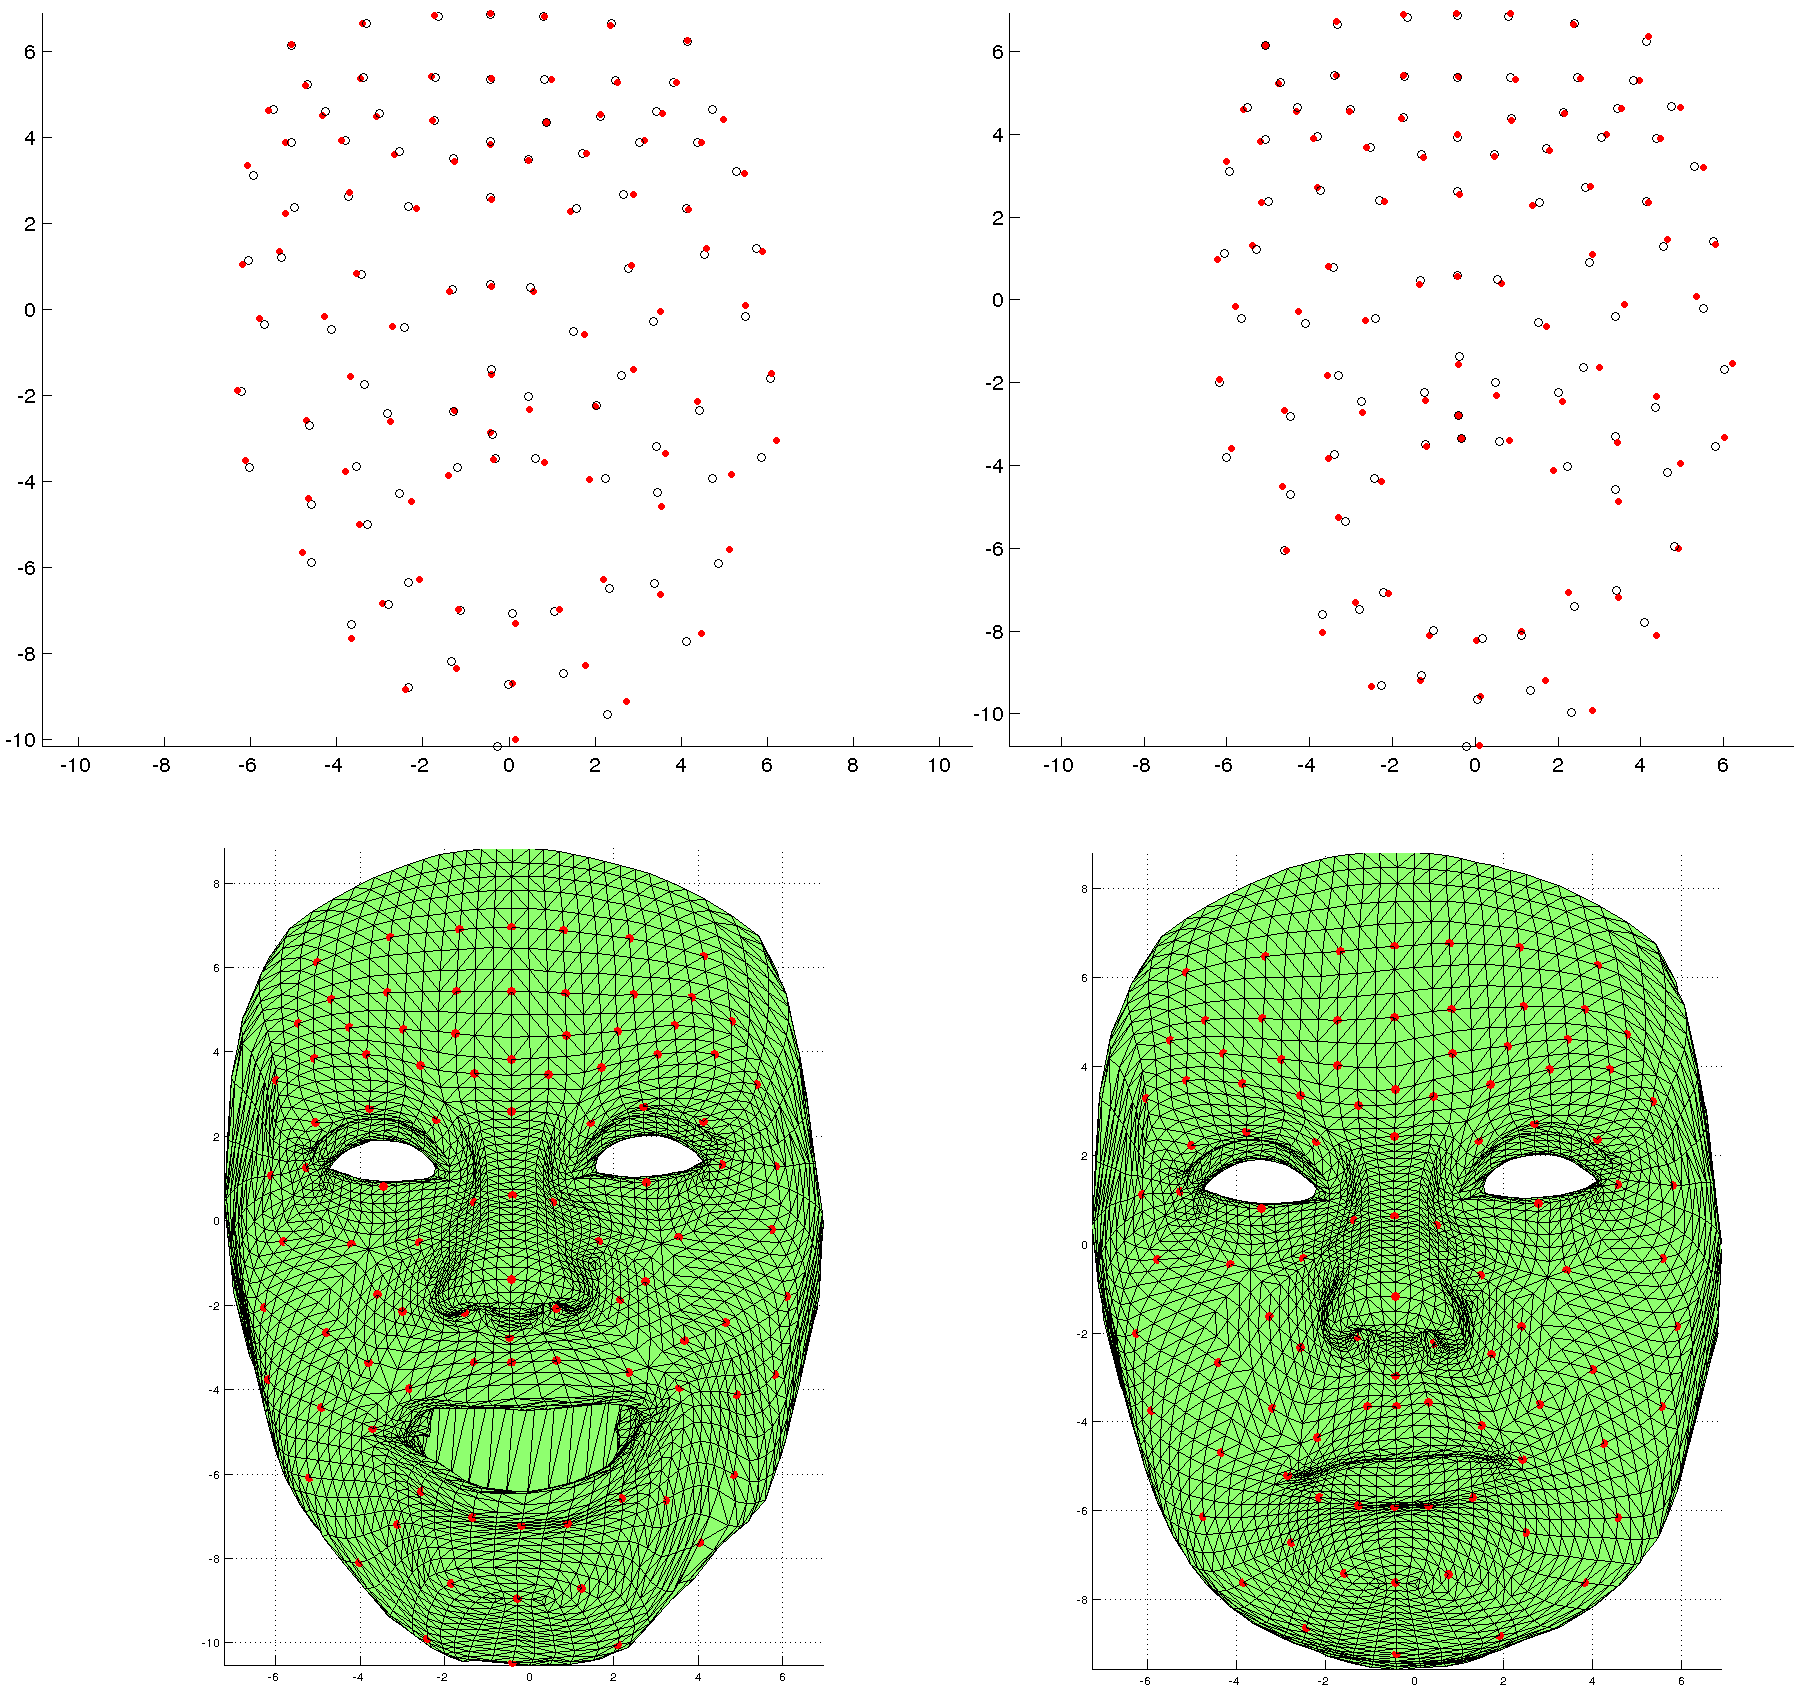
\includegraphics[width=\textwidth]{img/Emilydomain}
                \caption{Emily sequence}
        \end{subfigure}
\end{figure}}

\visible<2->{\begin{figure}
\centering

\includegraphics[width=0.5\textwidth]{img/backarrow}
\end{figure}}

\end{frame}
%----------------------------------------------------------------------
\section{Garoe's Part}
\begin{frame}{Frame name}

\end{frame}


\begin{frame}{Frame name}

\end{frame}


%----------------------------------------------------------------------
\section{Results}
\begin{frame}{Frame name}
%\begin{center}
%\begin{figure}
%\movie[width=0.45\textwidth, autostart, loop]
%        {\includegraphics[width=0.25\textwidth]{img/arkanoid}}{img/arkanoid1.mov}
%~
%%,showcontrols
%\caption*{\tiny{Left shows rigid body physics, right shows crossplatform interaction.}}
%\end{figure}
%\end{center}
\end{frame}


\begin{frame}{Frame name}

\end{frame}



%\begin{center}
%\begin{figure}
%\includegraphics[width=0.5\textwidth]{img/6phongReflexion} ~
%\includegraphics[width=0.5\textwidth]{img/8phongShading}
%\caption*{\tiny{Left shows flat shading, right shows Gouraud shading.}}
%\end{figure}
%\end{center}
%
%\begin{itemize}
%\setlength\itemsep{0.5em}
%\item 
%\end{itemize}

%\begin{multicols}{2}
%\begin{figure}[b!]
%\includegraphics[width=0.4\textwidth]{img/cloth_directions}
%\end{figure}
%
%\vfill
%\columnbreak
%\vspace*{\fill}
%\small{where $F$ are Fresnel terms, $\eta$ are Fresnel coefficients, $g$ is a Gaussian lobe, $k_d$ is a scattering constant, $\gamma$ are Gaussian widths, $\theta_h = (\theta_i+\theta_r)/2$ and $\phi_d = \phi_i-\phi_r$. }
%\end{multicols}


%----------------------------------------------------------------------

\end{document}
